% !TEX TS-program = xelatex
% !TEX encoding = UTF-8 Unicode
\documentclass[10 pt,landscape]{article}
\usepackage{syntonly}
%\syntaxonly
\usepackage{xeCJK}
\setmainfont{[Helvetica.ttf]}
\setsansfont{Consolas}
\setCJKmainfont{[Alibaba-PuHuiTi-Regular.ttf]}
\setCJKsansfont{[Alibaba-PuHuiTi-Medium.ttf]}
\setCJKmonofont{[Alibaba-PuHuiTi-Bold.ttf]}

\usepackage{graphicx} %图片插入
\graphicspath{{figure/}}% 路径
\usepackage{multicol} %多栏\emph{}
\usepackage{color}%颜色
\usepackage{float}
%\usepackage{draftwatermark}
%\SetWatermarkText{无安书}
\linespread{1.5}
\usepackage{fancyhdr}  %页眉页脚
\pagestyle{fancy}
%\renewcommand{\sectionmark}[1]{\markright{\thesection\,#1}}
\fancyhf{}
\fancyfoot[RO]{\sf \textcolor{violet}{\thepage}}


\definecolor{b1}{RGB}{49,75,139}
\usepackage{titlesec}
\titlelabel{\thetitle .\hspace{3mm}}
\titleformat*{\section}{\color{b1} \sf}
\titleformat*{\subsection}{\color{b1}\sf \small}
\titlespacing{\section}{0pt}{*5}{*2.5}
\titlespacing{\subsection}{15pt}{*1.5}{*1.2}
\usepackage{geometry}
\geometry{paper=a4paper,landscape,
 left=12 mm,
 right=12 mm, 
 top= 8 mm,
 bottom=13 mm}

\usepackage{enumitem}
\setlist{noitemsep,itemindent=0pt,leftmargin=1.4em,nosep}
\setlist[itemize]{label*=\ding{223}}
\setlength{\tabcolsep}{3pt} % 表格列间宽度

%\providecommand{\sectionbox}[1]{{\fboxsep0.5em\hspace*{-1.5\fboxsep}%
% \fcolorbox{gray}{gray!3}{%
% \parbox{\columnwidth}{%
% \raggedright #1}}}
% \vspace{0.1mm}} %节的矩形框
\providecommand{\sectionbox}[1]
{\raggedright#1 
\vspace{0.1mm}
}
%%%%%%%%%%%%%%%%%%%%%%%%%%%%
\usepackage{xcolor}
\definecolor{blue}{RGB}{91,137,163}		
\usepackage{hyperref}
\hypersetup{
	pdfcreator={tsia},
	pdfborder=false,
	breaklinks=true,
	bookmarksopen=true,
	bookmarksnumbered=true,
	linkcolor=orange,
	urlcolor=blue,
	citecolor=blue,
	colorlinks=true,
	pdfauthor= tsia, 
	pdftitle=R language Cheat Sheet,
	pdfcreator=tsia
}

\usepackage{listings}
\definecolor{l_gray}{gray}{0.97}



\lstnewenvironment{R}[1][]
{\lstset{
  caption={[#1]{#1}},
	backgroundcolor=\color[RGB]{253,253,253},
	basicstyle=\tt,
	emphstyle = \tt,
	frame=shadowbox, rulesepcolor=\color{gray},
	xleftmargin=2mm,xrightmargin=4mm,
	framexleftmargin = 4mm,
	framexrightmargin = 3mm,
	language = R, 
	breaklines, columns=flexible
	}}{}
	
	
	
\renewcommand*{\thesection}{\Alph{section}}
\setlength{\parindent}{0pt}
\setlength{\parskip}{0pt}




%\columnseprule = 0.5pt % 横线宽度
\setlength\columnsep{15 mm} % 双栏间距  mm\


  \definecolor{a1}{RGB}{50,50,50}
\newcommand{\rcode}[2]{
   \begin{tabular}{p{0.48\linewidth} p{0.45\linewidth} }
 {\sf \textcolor{a1}{#1} }  &      #2  \\
   \end{tabular}
   \\
}

\newcommand{\Rcode}[2]{
   \begin{tabular}{p{0.34\linewidth} p{0.6\linewidth} }
 {\sf \textcolor{a1}{#1} }  &      #2  \\
   \end{tabular}
   \\
}
\renewcommand{\contentsname}{目录}
 \renewcommand{\listfigurename}{图}
 \renewcommand{\listtablename}{表}

 \renewcommand{\refname}{参考文献}
 \renewcommand{\abstractname}{摘要}
 \renewcommand{\indexname}{索引}
 \renewcommand{\tablename}{表}
 \renewcommand{\figurename}{图}
 \renewcommand{\lstlistingname}{code}
 \renewcommand{\lstlistlistingname}{R-Code}
\usepackage{makecell}

\begin{document}
\begin{multicols*}{3} % 三栏
   
   
  
   \begin{center}
   \begin{tabular}{lc}
 \makecell{
\includegraphics[width = 10mm]{wuan}  }&
   {\Large \color{blue} \sf R语言 卡片}\\
     无安书 &
    2021.01.15   \\
    \end{tabular}
  \end{center}
\tableofcontents
\lstlistoflistings
\section{帮助类和常用基础函数}
  
     \sectionbox{
       \rcode{help(topic)}   {  查看帮助文档} 
       \rcode{?topic}      { 同上,查看帮助}
       
      }
   
    
    
     \subsection{变量相关}
     
     \sectionbox{
     \rcode{ls()}   {显示当前的所有变量名}   
     \rcode{objects()} { 同上,为ls() 的别名  }
     \rcode{rm()} { 清除变量 }
     \rcode{remove()}  { 清除对象,rm() 的别名 }
     \rcode{str()}  { 显示变量的属性信息 }
     \rcode{class()} { 查看对象类别 }
     \rcode{rm(list = ls())} { 删除所有变量 }
     \rcode{ls(`package:pkg')} { 查看包中的函数列表 }
         
     }
      
   
   \subsection{其他函数}
     \sectionbox{
        \rcode{setwd()} { 设置工作路径 }
        \rcode{getwd()}  { 查询工作路径 }
        \rcode{options()} { 设置全局参数 }
        \rcode{getOption()} { 获取参数信息 }
        \rcode{library()} { 加载包 }
        \rcode{require()} { 加载包,返回逻辑值 }
        \rcode{R.home()} { 返回 R 的安装路径 }
        \rcode{options(repos = `')} { 设置镜像网站 }
        \rcode{chooseCRANmirror()} { 窗口界面设置镜像网站 }
        \rcode{data()} { 查看自带的数据集信息 }
        \rcode{install.packages()} { 下载并安装包 }
        \rcode{q()}  {退出}  
        \rcode{quit()}  {q() 的别名函数}
        
     }
      
      \section{基本数据类型} 
      
   
       \subsection{创建}
      \sectionbox{
        \Rcode{c()} { 创建向量 }
        \Rcode{form:to} { 创建整数向量 }
        \Rcode{seq(from,to)} { 创建整数向量,参数 by 控制步长,参数 length 控制长度  }
        \Rcode{rep(x,times)} { 重复 x 中的值,times 控制重复几次;
            参数 each, 控制每一个元素重复几次;参数 len 控制长度。}
         \Rcode{list()}  {  创建列表   }
         \Rcode{matrix()} { 创建矩阵 }
         \Rcode{array()}  { 创建数组 }
         \Rcode{data.frame()} { 创建数据框 }
         \Rcode{factor()} { 创建因子 }
         \Rcode{append()} { 追加数据,默认在末尾追加 }
         \Rcode{`' 或 “”} { 创建字符串 }
         \Rcode{assign()}  { 赋值操作(常用于编写函数过程中) }
         \Rcode{NA,NaN,} { 对应Not Available, Not a Number }
         \Rcode{Inf} {正无穷值,-Inf 代表负无穷}
         \Rcode{NULL} {The null objects}
         \Rcode{paste()}  { 连接字符串 }
         \Rcode{paste0()} { 等同于 paste(...,sep = `') }
             
       }
    
      
   
      \subsection{基本-内嵌变量名}
           \subsubsection{字母}
        \begin{R}[letters]      
> letters
 [1] "a" "b" "c" "d" "e" "f" "g" "h" "i" "j" "k"
[12] "l" "m" "n" "o" "p" "q" "r" "s" "t" "u" "v"
[23] "w" "x" "y" "z"
> LETTERS
 [1] "A" "B" "C" "D" "E" "F" "G" "H" "I" "J" "K"
[12] "L" "M" "N" "O" "P" "Q" "R" "S" "T" "U" "V"
[23] "W" "X" "Y" "Z"
       \end{R}   
     \vspace{3cm}
     \subsubsection{月份}
            \begin{R}[month] 
> month.abb
 [1] "Jan" "Feb" "Mar" "Apr" "May" "Jun" "Jul"
 [8] "Aug" "Sep" "Oct" "Nov" "Dec"
> month.name
 [1] "January"   "February"  "March"    
 [4] "April"     "May"       "June"     
 [7] "July"      "August"    "September"
[10] "October"   "November"  "December" 
       \end{R}
     \subsubsection{其他常量数据}
     \begin{R}[常量型数据]
> 1i   #复数
[1] 0+1i
> pi  
[1] 3.142
> 1e-5 #科学计数法,也可表示为: 1E-5
[1] 1e-05
> 2 + 3i #复数
[1] 2+3i     
     \end{R}
     
     \subsection{逻辑值}
     
     \begin{R}[逻辑值]
> T
[1] TRUE
> F
[1] FALSE
> TRUE
[1] TRUE
> FALSE
[1] FALSE

     \end{R}
     
      \section{输入与输出}
      
      \sectionbox{
        \Rcode{print()}  {打印输出}  
        \Rcode{cat()}  {输出} 
        \Rcode{sink(file)} {输出之后的内容至文件,直至 输入 sink() 结束}
        \Rcode{edit(x)}  {修改变量}
        \Rcode{fix(x)} {修改变量}
        \Rcode{x <- scan()}  {从键盘上输入数据}
       
      } 
      \sectionbox{
       \Rcode{read.table()} {读取数据,分隔符为空格}
        \Rcode{read.csv()} {读取 csv 型数据,分隔符为 逗号}
        \Rcode{save()} {保存输出} 
        \Rcode{load} {加载数据}
        \Rcode{attach()} {绑定数据集}
        \Rcode{detach()} {解绑数据集}
        \Rcode{history()} {\makecell[l]{输出历史记录,搭配 Inf,\\ 利用 history(Inf),输出所有历史记录}}
        \Rcode{savehistory()} {保存历史记录}
        \Rcode{saveRDS()} {保存输出} 
        \Rcode{readRDS()} {读取}
        \Rcode{readLines()} {读取行}
        \Rcode{wirteLines()}{输入至行}
        \Rcode{.Last.value}{上一个结果显示}
        \Rcode{read.delim(`clipboard')}  {}
        \Rcode{read.fwf()}  {读取固定宽度格式文件}
      }
      
      \section{变量-相关函数}
      \sectionbox{
        \Rcode{ is.xxx()}  {is. 系列判断是否为某一类型变量}
        \Rcode{as.xxx()} {as. 系列函数用于转换变量类型}
        \Rcode{ methods('is')} {显示上述的is 系列函数列表}
        \Rcode{methods('as')}  {同上}  
        \begin{tabular}{lll}
         as.numberic(x)  &  as.integer(x) & as.character(x) \\
         as.logical(x)  &  as.data.frame(x)  & as.factor(x)  \\
         is.numeric(x) & is.null(x)  & is.na(x)  \\
         
        \end{tabular}\\
      }
      \begin{R}[查询变量类型的方式]
> a <- 1:5
> mode(a)
[1] "numeric"
> str(a)
 int [1:5] 1 2 3 4 5
> class(a)
[1] "integer"
> typeof(a)
[1] "integer"
      \end{R}
      {\sf a<- 1:5}
      mode(), str(), class(), typeof() 均可用于查询变量的属性信息,但有所差别。
      \begin{R}[属性]
> names(a)
NULL
> attributes(a)
NULL
#names() 查询 name 属性,attributes() 显示变量属性
      \end{R}
      
      \sectionbox{
       \Rcode{length(x)}  {返回变量的长度}
       \Rcode{dim(x)}  {返回变量的维度信息}
       \Rcode{\makecell[l]{nrow(x)\\ncol(x)}} {返回行数、列数}
       \Rcode{unname(x)}  {移除 name 属性}
      }
      \subsection{向量-索引}
        \sectionbox{
          \Rcode{x[n]}  {第n 个元素}
          \Rcode{x[-n]}  {去除第 n 个元素后的变量}
          \Rcode{x[m:n]}  {第 m 个到第n 个元素}
          \Rcode{x[c(1,4,2)]} {指定序号位置的元素}
          \Rcode{x[-c(1,4,2)]} {去除指定序号的元素}
          \Rcode{x[x > 5]}  {值大于 5的元素,类似地有:<, <=, >= !=}
        
        \Rcode{x[x>4 \& x<8]} {值 在 4到8之间的元素}
      }
      \subsection{向量-必要操作}
        \sectionbox{
         \Rcode{rev(x)} {颠倒向量中的元素}
         \Rcode{unique(x)}  {返回向量中的唯一值}
         \Rcode{duplicated(x)}  {返回向量中的重复值}
         \Rcode{table(x)} {返回频数表}
         \Rcode{sort(x)}  {升序排列}
        }
      \section{数学相关函数}
    
        \sectionbox{
          \rcode{+,-, x,/} {对应$+,-,\times,\div$ }
          \rcode{\^{},\%\%,\%/\%} {对应开方,余数,整除}
          \rcode{\makecell[l]{sin(x),cos,tan,\\asin,atan,acos}} {三角函数}
          \rcode{\makecell{sinpi(x);\\cospi,tanpi}} {等同于 sin(pi*x)...}
          \rcode{abs(x)} {绝对值}
          \rcode{sign(x)} {根据正负返回 1或 -1;0 }
          \rcode{min(x);max(x)} {最小值,最大值}
          \rcode{median(x)} {中位数}
          
          \rcode{range(x)}  {返回 c(min(x),max(x))}
          \rcode{sqrt(x)}  {开根}
          \rcode{sum(x)} {求和}
          \rcode{var(x)} {方差}
          \rcode{sd(x)} {标准差, = sqrt(var(x))}
          \rcode{\makecell[l]{log(x,\\base = exp(1))}} {取对数,默认以e为底}
          \rcode{log10(x)} {以10为底的对数}
          \rcode{log2(x)}  {以2为底的对数}
          \rcode{log1p(x)} {= log(1+x)}
          \rcode{exp(x)} {$e^x$}
          \rcode{expm1(x)}  {$e^x -1$ } 
          \rcode{fivenum(x)} {五个分位数汇总}
          \rcode{\makecell{quantile(x,\\probs = )}} {分位数输出}
          \rcode{IQR(x)} {中间 50\% 的范围大小}
          \rcode{cov(x,y)}  {协方差}
          \rcode{cor(x,y)}  {相关系数}
          \rcode{var(x);cov(x)} {样本方差}    
       }
       
       \sectionbox{
               
           \rcode{prod(x)}  {连乘}
          \rcode{cumprod(x)} {连乘}
          \rcode{diff(x)}  {差分,返回 x[i+1] - x[i]}
         \rcode{factorial{n}} {阶乘 n!}
         阶乘的计算方法汇总:\\
         factorial(n) \quad  gamma(n+1) \quad  prod(1:n) 
         \\
         \rcode{ployroot(c(2,-3,1))}  {求 $2 -3x+x^2 =0$根} 
         uniroot(function(x) x\^{}2 - x\^{}3, c(-3,2))\\
         \hspace{3.5cm}$x^2-x^3 =0$ 在 [-3,2]范围内的根
          D(quote(x\^{}2+sqrt(x/(x+1))),'x')\\
         \hspace{3.5cm}求 $x^2 +\sqrt{\frac{x}{x+1}}$ 的导数
          \\
         
       }
        
        \sectionbox{
         
         also: \\
          a <- D(quote(sin(x*y)+ tan(x/(x+y))),'x') \\
          eval(a,list(x =4,y = 7))  \quad  对x 进行单独求导,y作为常数先求导,后用 eval() 进行求导后的计算。
          \\
          积分:
          integrate(function(x) 2*x+ sin(x\^{}2) + tan(x/(x+1)) ,0, 1) \\
            \hspace{1cm} 从[0,1] 范围对 $y = 2x + \sin{x^2} + \tan{\frac{x}{x+1}}$ 进行积分 \\
            多项式极值:\\
       f <- function(x)  2*x+ sin(x\^{}2) + tan(x/(x+1))\\
optimize(f,c(-4,10)) \#区间[-4,10]内的最小值 \\
optimize(f,c(-4,10),maximum= T)\#求最大值\\ 

        
        }
       
        上述代码运行结果如下所示:
        \begin{R}[求导,积分,极值计算]
> D(quote(x^2+sqrt(x/(x+1))),'x')
2 * x + 0.5 * ((1/(x + 1) - x/(x + 1)^2) * (x/(x + 1))^-0.5)
> a <- D(quote(sin(x*y)+ tan(x/(x+y))),'x') ;
> eval(a,list(x =4,y = 7)) 
[1] -6.672
> integrate(function(x) 2*x+ sin(x^2) + tan(x/(x+1)) ,0, 1)
1.633 with absolute error < 1.8e-14
> f <- function(x)  2*x+ sin(x^2) + tan(x/(x+1))
> optimize(f,c(-4,10))
$minimum
[1] -2.752

$objective
[1] -75038

> optimize(f,c(-4,10),maximum= T)
$maximum
[1] 8.78

$objective
[1] 19.81
        \end{R}
        
        \subsection{集合运算}
     \sectionbox{
      \Rcode{union(x,y)}  {并集}
      \Rcode{intersect(x,y)}  {交集}
      \Rcode{setdiff(x,y)} {差集}
      \Rcode{setequal(x,y)} {是否相等}
      \Rcode{identical(x,y)} {检查是否完全相等}
     }
     
     \subsection{其他函数}
       \sectionbox{
       \Rcode{set.seed(x)}  {设定随机数种子}
        \Rcode{sample(x,n)} {从 x 中随机取出 n 个元素,不放回抽样。replace = T, 则为放回抽样}
        \Rcode{choose(n,k)}  {{\LARGE$\frac{n!}{(n-k)!k}$}一共有多少种组合}
        \Rcode{combn(x,m)} {组合数列表显示}
        \textcolor{blue}{\sf 平均值系列:}
        \rcode{mean(x)}  {平均值}
          \rcode{mean(x,trim=0.1)} {去头去尾,求平均值} 
          \rcode{weighted.mean(x,w)}  {加权平均值}
       }
     \section{向量操作}
       \sectionbox{
        \Rcode{which.max(x)} {返回最大值的索引}
        \Rcode{which.min(x)}  {返回最小值的索引}
        \Rcode{which(x == y)} {返回相等的值的索引}
          \Rcode{pmax(x,y,...)} {返回对应序号的最大值,组成新的向量}
          \Rcode{pmin(x,y,...)}  {同上,但返回最小值}
        
       }
       
       \sectionbox{
       \Rcode{cumsum(x)} {累加,返回新的向量 x[i]= sum(x[1:i])}
       \Rcode{cumprod(x)} {累乘,同上}
       \Rcode{cummin(x)} {最小值}
       \Rcode{cummax(x)} {最大值}
       }
       \begin{R}[cum 系列]
>  y <- c(2,4,3)
>  cumsum(y)
[1] 2 6 9
>  cumprod(y)
[1]  2  8 24
> cummin(y)
[1] 2 2 2
> cummax(y)
[1] 2 4 4
       \end{R}
      \section{字符串处理}
         \subsection{基础函数}
             \rcode{paste()}  {连接字符串,参数sep = `` '',默认连接时以空格作为分隔}
             \rcode{paste0()} {连接字符串,但不产生分隔}
             \rcode{nchar(x)}  {统计字符个数,与 length() 不同}
             \rcode{strsplit(x,split} {在 split 指定的位置对字符进行分割}
             \rcode{\makecell[l]{sub(pattern,\\replacement,x)}}  {替换字符}
             \rcode{gsub()}  {同上,但替换所有满足条件的字符}
             \rcode{chatr(old,new,x)}  {替换字符,old 内容改为 new}
             \rcode{substr(x,start,stop)}  {提取指定位置的字符片段}
             \rcode{casefold(x,upper =T)} {改为大写。upper =F 时,改为小写}
             \rcode{toupper()}  {改为大写}
             \rcode{tolower()}   {改为小写}
             首字母大写:\\
              \rcode{Hmisc::capalize()} {首字母大写}
              \rcode{\makecell[l]{stringr中的\\ str\_to\_title()}} {首字母大写}
              \rcode{noquote(`a')} {去除引号}
              \rcode{quote()} {}
              \rcode{sprintf()} {字符格式化}
           sprintf(``...\%d...'',x)   常见格式化: \%d,\,\%f,\,\%m.nf 等
           \rcode{trimws(x)}  {清除字符串首尾空白}        
           \rcode{\makecell[l]{Encoding(x) <- \\`UTF-8'}}  {UTF-8 编码,类似地,也可以选择 GB2312 编码方式}
           \rcode{iconv(x,...)} {转换编码方式}
           
         \subsection{stringr 包}
      \section{日期}
        \sectionbox{
           
         \Rcode{weekdays(x)}  {返回日期对应的星期几} 
         \Rcode{months(x)}  {返回月份}
         \Rcode{quarters(x)}  {返回第几季度}
         \Rcode{as.Date(x)}  {转为日期}
         \Rcode{as.POSIXct(x)} {转为日期时间}
         \Rcode{timestamp()} {返回当前时间}
       \Rcode{   {\sf\textcolor{blue}{日期格式:} } }
       { 以 2021.01.21\,11:12:30 为例}
         \Rcode{\%Y} {年份,2020}
         \Rcode{\%y}  {年份,00-99}
         \Rcode{\% m} {月份,01-12}
         \Rcode{\%b} {缩写的月份名}
         \Rcode{\%B} {月份名}
         \Rcode{\%d} {日期 01-31}
         \Rcode{\%j} {一年中第几天}
         \Rcode{\%U} {一年中第几个星期,00-53,以星期天作为一周的开始}
         \Rcode{\%W} {同上,但以星期一作为一周的开始}
         
         \Rcode{\%w} {星期几,0-6,周日为0}
         \Rcode{\%a} {星期几的名称,缩写}
         \Rcode{\%A} {同上,但为全称}
         \Rcode{\%H} {小时,00-23}
         \Rcode{\%I} {小时,01-12}
         \Rcode{\%p} {AM,PM,可与 \%I 搭配使用}
         \Rcode{\%M} {分钟,00-59}
         \Rcode{\%S} {秒}
        }
      \section{数据框-操作}
      \section{拟合-获取线性拟合结果}
         \subsection{线性拟合}
         \sectionbox{
           \rcode{lm(y\~{}x)}  {返回线性拟合结果}
           \rcode{lm(y\~{}x, data = df)} {y与 x 来自数据框 df }
           \rcode{lm(y\~{}x - 1)}  {截距为零的拟合}
           \rcode{fit  <-lm(y\~{}x)}  {赋值给变量,fit}
           \rcode{confint(object, parm, level = 0.95, ...)} {求置信区间,默认:0.95}
           \rcode{summary(fit)} {汇总拟合结果}
           \rcode{coef(fit)}  {返回模型系数}
         }
         
         \begin{R}[模型拟合]
set.seed(5)
x <- 1:5 + sample(1:10,5) * 0.01 
y <- 2 *x + sample(1:20,5) * 0.023
m <- lm(y ~ x)
lm(y ~ x -1)
confint(m)
names(m)
residuals(m)         
         
         \end{R}
         
         \subsection{model formulas} 
    \sectionbox{
       y \~{} x1 + x2 + a + b + ... \\
       操作符汇总:
       \Rcode{\~{}}  {分隔符}
       \Rcode{1} {截距项为零} 
       \Rcode{-}  {移除某一个变量}
       \Rcode{:} {交互项,如 a:b}
       \Rcode{*} {所有可能的交互项, a*b 表示 a + b + a:b}
       \Rcode{\^{}} {乘方,如 a\^{}2}
       \Rcode{.}   {除因变量以外的所有变量,  lm(y \~{} . data =) }
       \Rcode{I()}  {解释变量, y \~{} x + I(x\^{}2)}
    }
        
  \begin{R} [多项式回归 ]
      
model <- lm(y ~ poly(x,3,raw = T))
model_2 <- lm(y ~ x + I(x^2) + I(x^3) )
\end{R}   
      
      \section{操作符}
        
          \Rcode{?Syntax}  {操作符优先顺序}
           \Rcode{:: and :::}  {命名空间中的变量,多用于包中的函数的直接调用,如 pkgname::function, 后者调用包中的未声明函数}
          \Rcode{ \$}  {提取变量中的子集}
          \Rcode{[  and [[} {提取元素}
          \Rcode{\^{}}  {指数}
          \Rcode{:}  {用于生成序列}
          \Rcode{\%\%  \%/\%}  {整除,余除}
          \Rcode{* /}  {乘、除}
          \Rcode{$+ \, -$}  {二元运算的加减}
          
          \Rcode{\makecell{< > <= >=\\ == !=}	} {比较运算符}
          \Rcode{!}  {非}
          \Rcode{\& \&\&} {与}
          \Rcode{|  ||} {或}
          \Rcode{\~{}}  {用于 formula 中}
          \Rcode{-> ->>	}  {右向赋值}
          \Rcode{<- <<-}  {左向赋值}
          \Rcode{=} {同上,但优先级低}
          \Rcode{?}  {查询帮助}
          
          \vspace{5 mm}
    关于赋值:\\
      \begin{tabular}{ll}
       ->  & -> > \\
       <-  & < <- \\
       = & assign() \\
      \end{tabular} \newline
      共计六种赋值方式,但 = 用于给参数赋值,-> 和 <- 赋值使用较多,而 -> > 和 < <- 用于全局变量的赋值; assign() 用于编写函数过程中的赋值语句。
      \subsection{二元运算符}
      
        \Rcode{\%in\%}  {是否含于}
           \begin{R}[\%in\%]
> a <- c(1,4,3,6,7)
> 3 %in% a
[1] TRUE
> c(1,3,5) %in% a
[1]  TRUE  TRUE FALSE
           \end{R}
      \subsection{逻辑运算的比较}
         \& 和 |  \quad 作用于对象的每一个元素 \\
         \&\& 和|| \quad 只作用于对象的第一个对象\\
    
    \section{packages 相关}
      \begin{R} [以 .packages 结尾的函数名]
> apropos('\\.packages') %>% print(quote = F)
 [1] .packages              
 [2] .packageStartupMessage 
 [3] .rs.packages.initialize
 [4] .rs.packagesLoaded     
 [5] available.packages     
 [6] CRAN.packages          
 [7] download.packages      
 [8] install.packages       
 [9] installed.packages     
[10] make.packages.html     
[11] new.packages           
[12] old.packages           
[13] remove.packages        
[14] update.packages 
      \end{R}
      以上函数中常用的为:.packages(),  download.packages(), install.packages(), installed.packages(), old.packages(), remove.packages(), update.packages()
      \rcode{\makecell{search()\\ (.packages())}}  {显示已加载的包}
      \rcode{ \makecell{library() \\  require()}  }    {加载包}
      \rcode{.libPaths()}  {包的安装路径顺序}
      \rcode{.Library}    {目录地址}
      \rcode{ls(`package:pacman‘)} {查看 pacman 包中的函数}
      
      \rcode{\makecell[l]{detach(`package:pkg’) \\
        unloadNamespace(`pkg‘)} }  {\makecell{解绑该包}}
      \rcode{remove.packages()}  {卸载包}
      \rcode{install.packages()}  {下载包 }
      \rcode{old.packages()} {已安装的包中为旧版本的包列表}
      \rcode{update.packages(ask = F)} {不再询问,选择全部更新包}
      \rcode{ \makecell[l]{pkgs = installed.packages()\\
      colnames(pkgs)\\
      str(pkgs)\\
      c(`pkg1`,`pkg2`,...) \%in\% pkgs\$package}}  {\makecell{查询已安装包的信息}}
      \rcode{getOPtion(`defaultPackages`)} {}
      \rcode{system.file()} {base 包的目录}
      \rcode{\makecell{system.file(pac\\kage = `ggplot2`)}}  {ggplot2 的目录位置}
      
      \section{颜色}
         \rcode{palette()} {默认调色板}
         \rcode{col2rgb()} {颜色转为 RGB 模式}
         \rcode{colors()} {默认支持的颜色列表} 
       \begin{R}[究竟有多少种唯一的颜色]
> length(colors())
[1] 657
> colors() %>% col2rgb %>% t %>% unique %>% nrow
[1] 502
\end{R}      
657 种颜色中,502 种为唯一值
      \rcode{scales::show\_ col(colors(),F)} {返回颜色的可视化显示}
      
     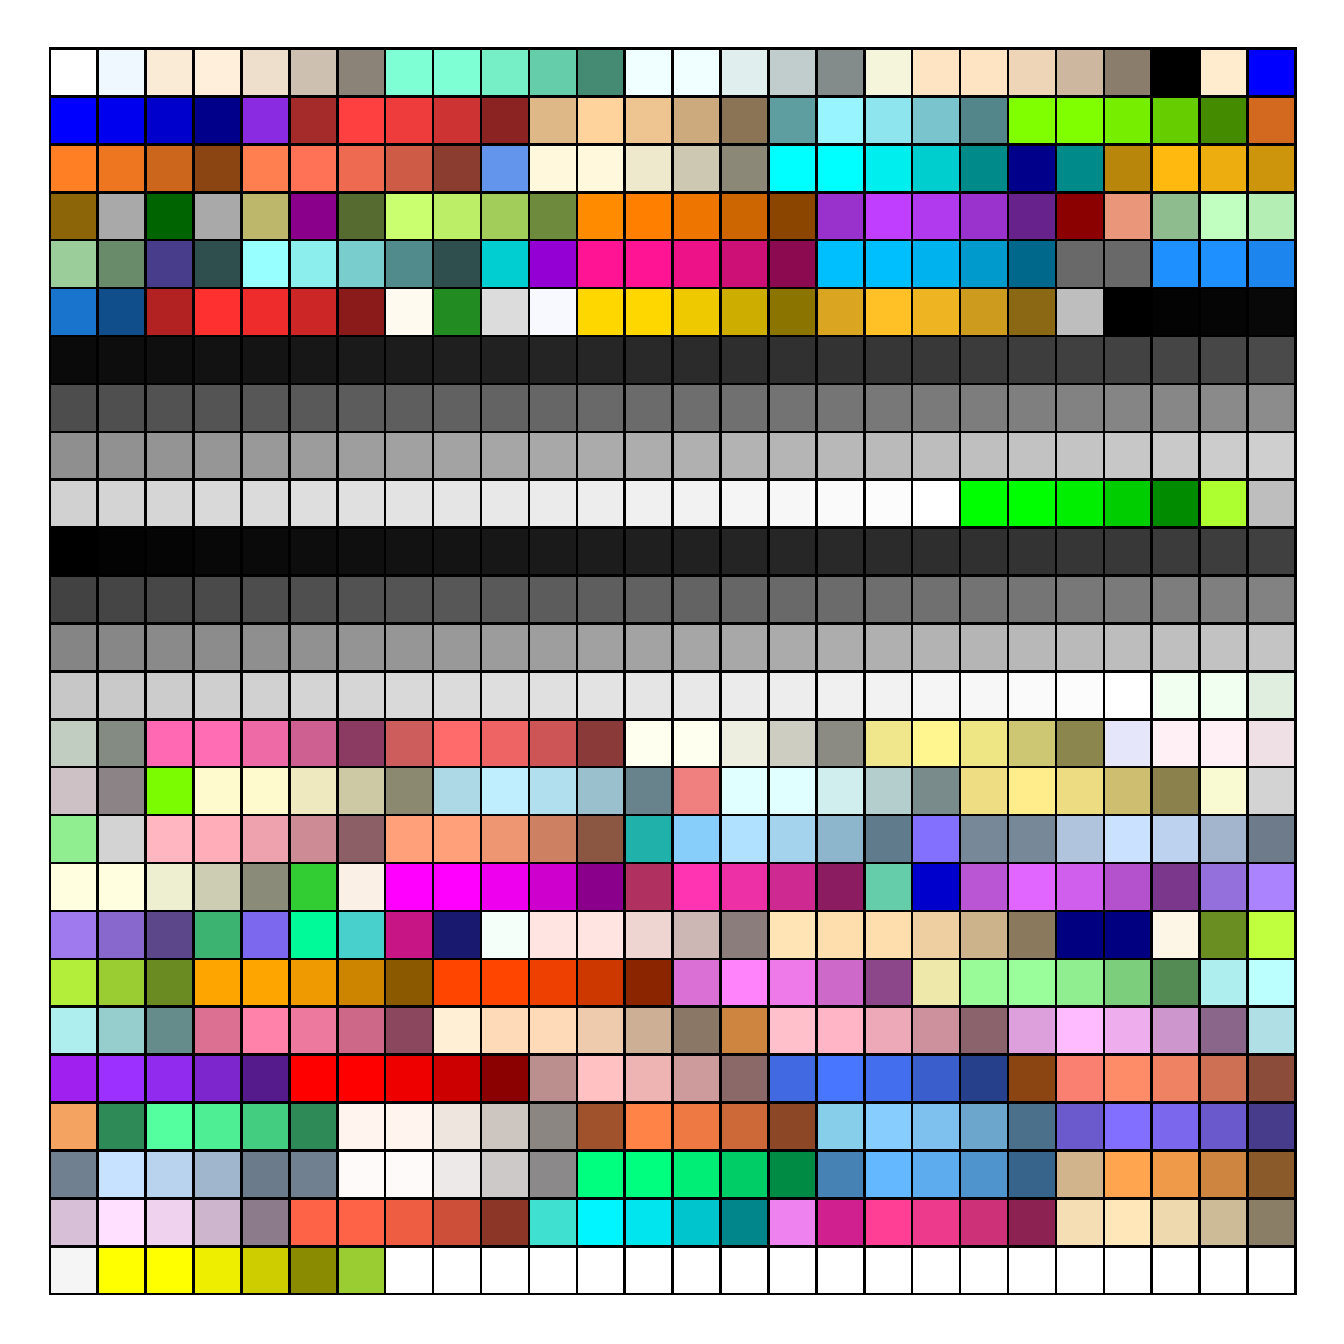
\includegraphics[width = 0.95\linewidth] {showcol} 
     
     \begin{R}[自制 ggplot2 绘图-显示颜色]
p1 <- show_color(colors(), 20,label = T,number = T)
p2 <- show_color(colors(),20,byrow = F,label =T, number =T)
p1
ggsave('showcolor1.pdf', width = 8, height = 7, unit = 'cm',scale = 4)
p2
ggsave('showcolor2.pdf', width = 8, height = 7, unit = 'cm',scale = 4)
\end{R}
        \begin{figure}[H]
          \centering
       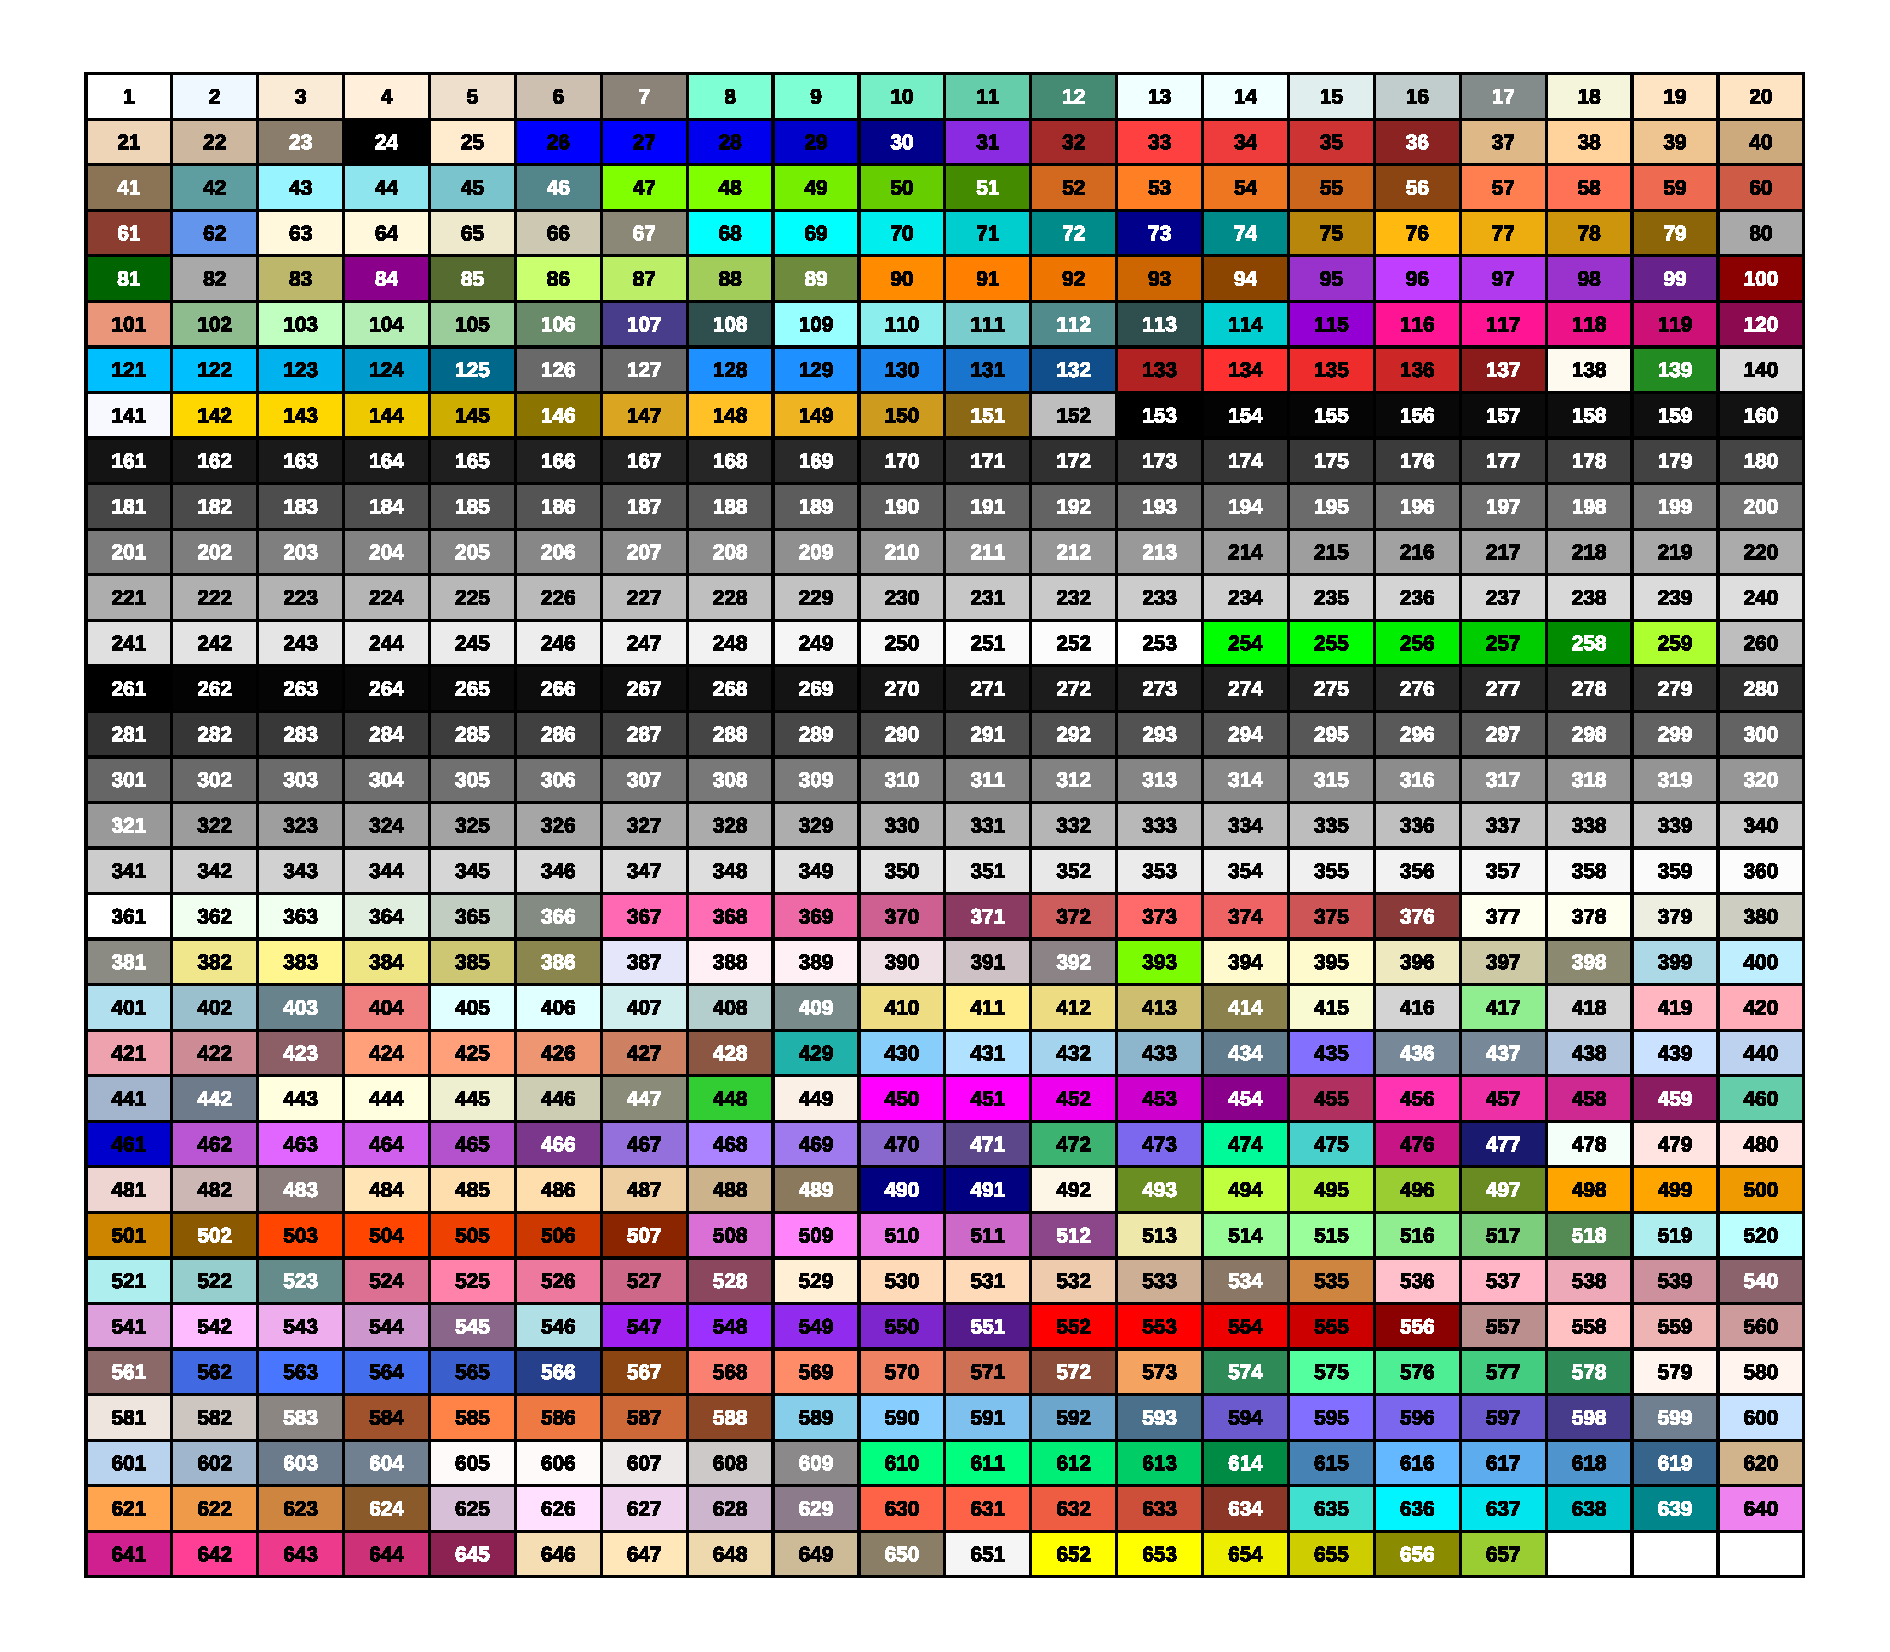
\includegraphics[width =1.1 \linewidth] {showcolor1} 
         \caption{byrow = T}
       \end{figure}
       
         \begin{figure}[H]
          \centering
       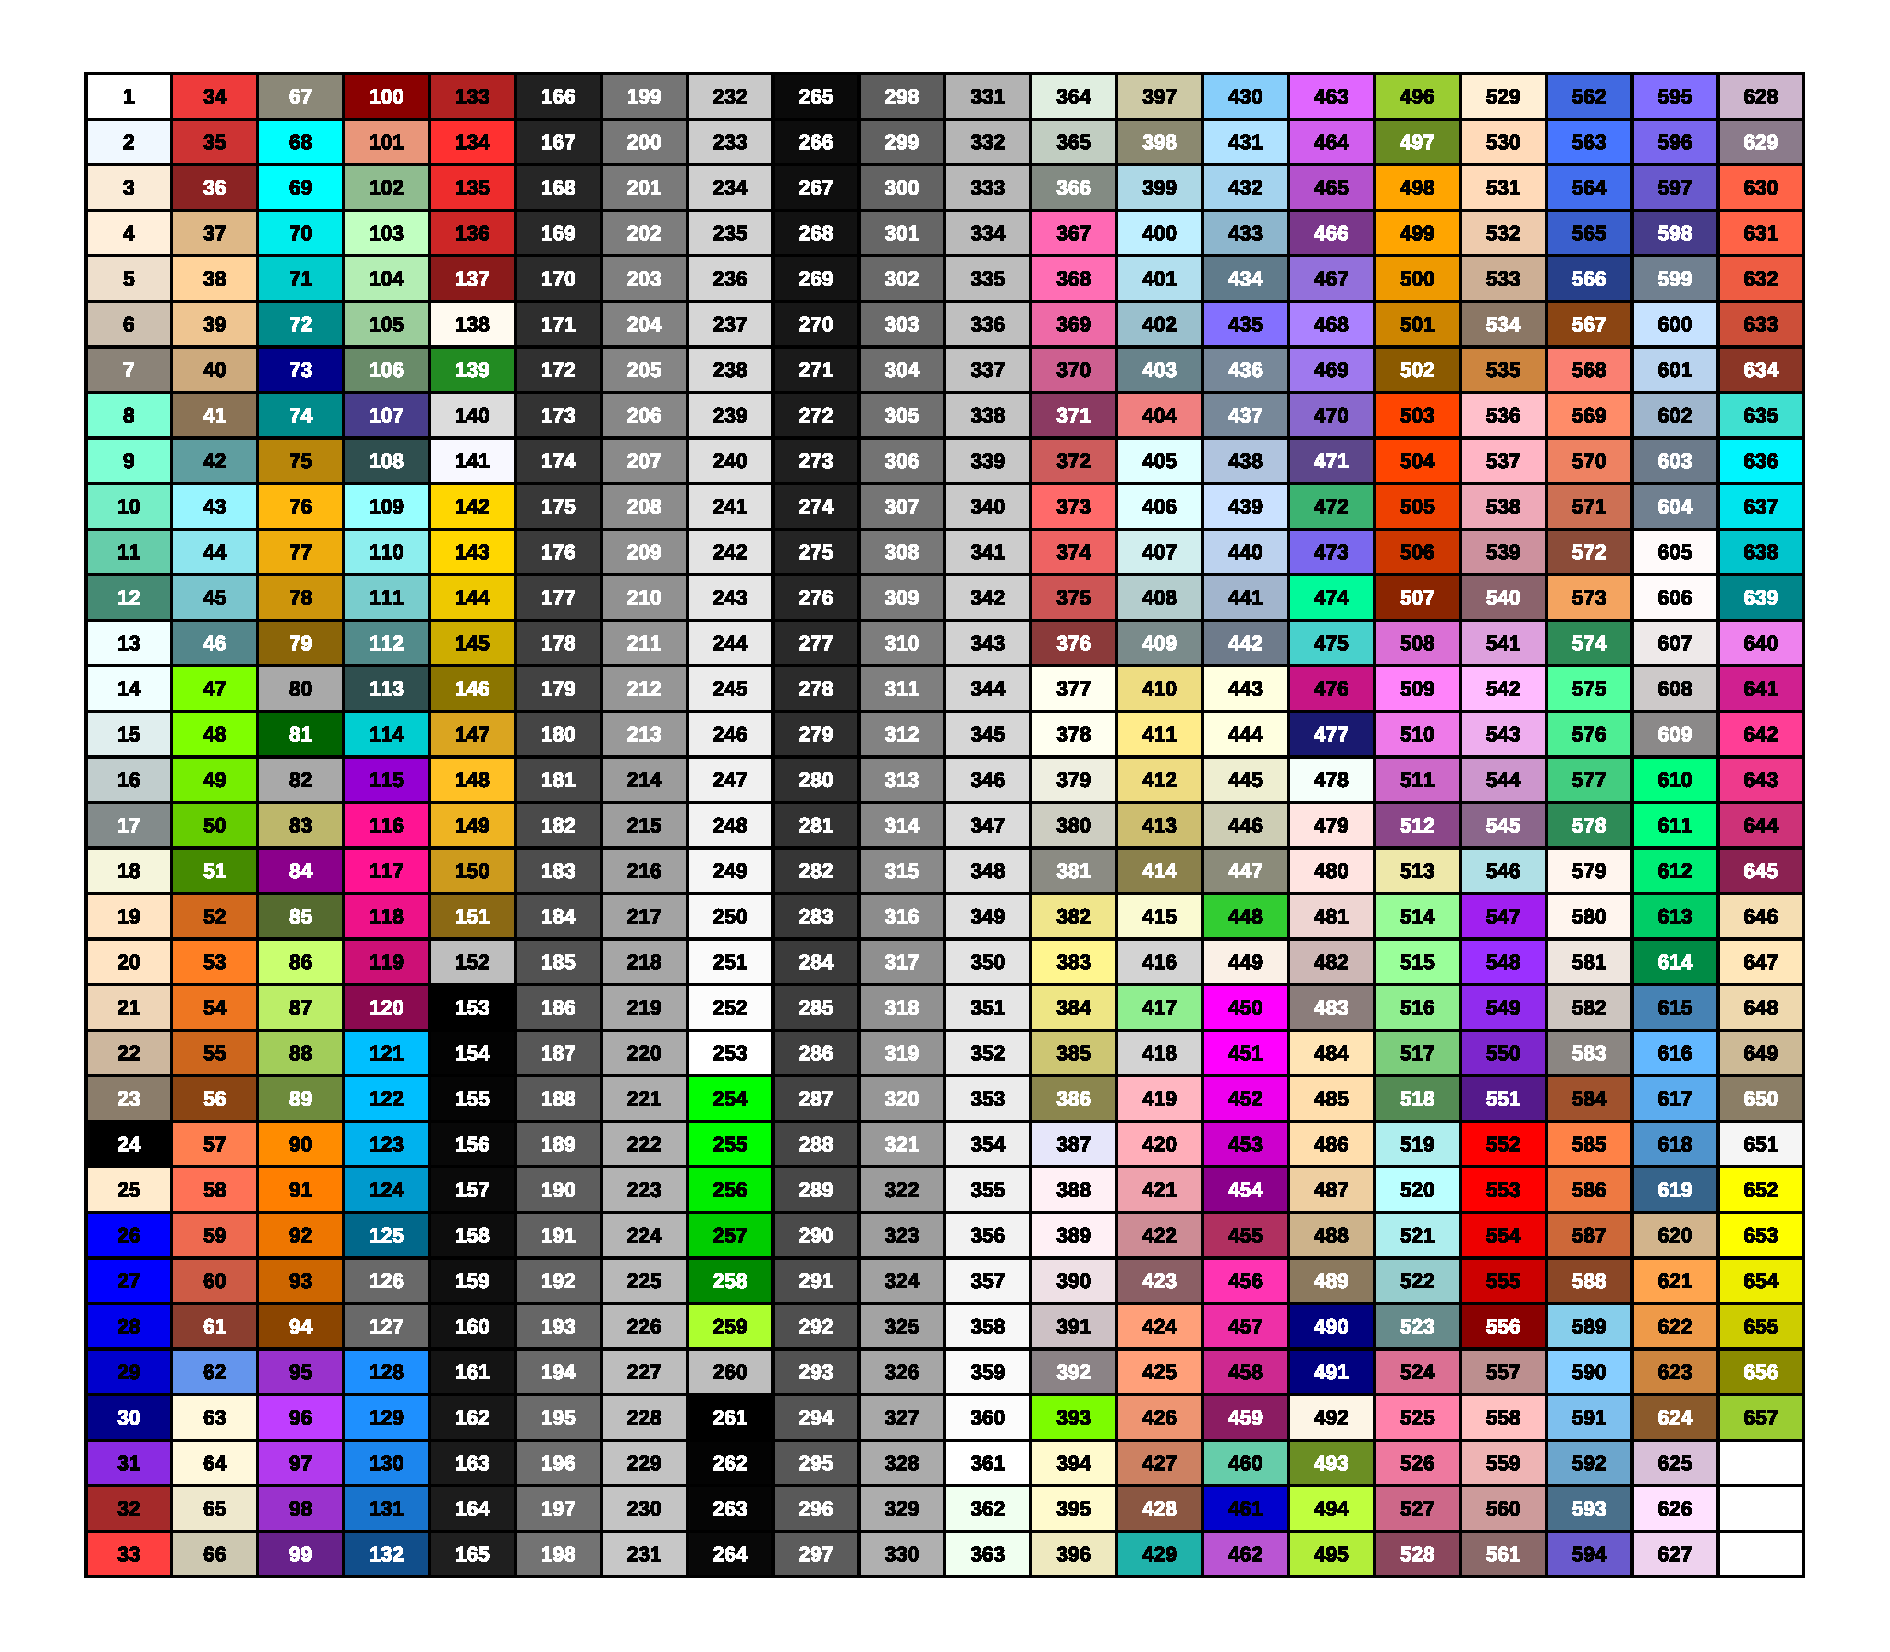
\includegraphics[width =1.1 \linewidth] {showcolor2} 
         \caption{byrow = F}
       \end{figure}
       
        \section{批处理与分组计算}
       \subsection{apply族函数}
          \rcode{apply(x,MARGIN,FUN=)} {x多为数据框,MARGIN:按行或按列计算,1:行,2:列;FUN:调用函数}
         \rcode{lapply(x,FUN=,...)}  {x 为列表、数据框,FUN:调用函数,返回值为列表,对数据框的列进行计算}
         \rcode{sapply()}   {lapply() 的简化版函数,参数 simplify = TRUE}
        \rcode{mapply()}  {多变量的 sapply() 函数}     
        \rcode{\makecell{tapply(x,INDEX,FUN=,\\...,simplify = T)}}  {分组计算} 
        \rcode{\makecell{lapply(file,\\read.table)}} 
        {\makecell{针对多个文件名的向量\\进行读取数据,\\输出为列表}} 
      
      \subsection{分组计算}
      
     \rcode{\makecell{ aggregate(x,by,FUN,\\,...
        simplify =T)}}     {分组统计}
       \rcode{\makecell{aggregate(formula,\\data,FUN,...,
       subset)}}  {\makecell{\\[6mm]分组计算,\\使用 formula 形式}}
       \rcode{\makecell{group\_by()\\ summarise()}}
         {搭配使用,源自 dplyr 包}
         
     \section{目录及文件操作}
        \rcode{setwd()}   {设置工作目录}
        \rcode{getwd()}  {获取工作目录}
        \rcode{file.choose()}  {弹出窗口,选择文件}
        \rcode{choose.dir()}    {弹出窗口,选择文件夹}  
        \rcode{list.dirs()}    {返回目录下的子目录内容}
        \rcode{dir()}  {返回选定路径下的子目录和文件名}
        \rcode{list.files()} {同 dir().参数 recursive = T时,可显示子目录内容}
        \rcode{dir.create()} {创建目录。参数 recursive =T时,可创建多级目录} 
        \rcode{file.create()}   {创建空的文件}
        \rcode{dir.exists(path)} {判断路径 是否存在}
        \rcode{file.exists()}  {判断文件是否存在}
        \rcode{file.remove()}   {删除文件,\textcolor{red}{谨慎操作,此操作后文件不进入回收站,无法复原}  }
        \rcode{file.rename()}   {修改文件名}
        \rcode{file.copy()}  {复制文件}
        \rcode{\makecell[l]{ file.info() \\ file.size() \\ file.mtime() }  }     { 文件信息获取}
        \rcode{R.home()}  {R 的安装路径}
        \rcode{system.file()}  {查看包的安装路径}
        \rcode{\makecell[l]{file.path(`a',\\`b',`d')}} {返回“a/b/d”,用于创建多级路径}   
        \rcode{normalizePath(path)}  {标准化路径}
        \rcode{shortPathName()}  {返回短路径}
        \rcode{dirname()}  {返回除文件名以外的路径}
        \rcode{zip()}  {创建压缩文件}
        \rcode{unzip()}  {解压缩}
        \rcode{apropos(`file \textbackslash \textbackslash.')} {返回 file. 开头的函数名}
        \begin{R}[file.开头的函数名]
> apropos('file\\.')
 [1] "file.access"  "file.append"  "file.choose" 
 [4] "file.copy"    "file.create"  "file.edit"   
 [7] "file.exists"  "file.info"    "file.link"   
[10] "file.mode"    "file.mtime"   "file.path"   
[13] "file.remove"  "file.rename"  "file.show"   
[16] "file.size"    "file.symlink"    
        \end{R}
        
         file.append() 在文件后面扩充,但没有从头扩展的函数。对于想要在文件开头添加内容的需求,可以换个法子,先读取,后写入新内容,再在后面 扩充就内容,实现曲线救国。\\
        \rcode{file.edit()}{修改文件}
        
    \section{表达式-expression}
    \begin{R}
    c('x %*% y' , 'x %/% y',  'alpha',  'sigma',  'beta'  ,
  'x == y',  'frac(x,y)',  'x %up% y',  'hat(x)',
  'symbol(a)','underline(x)') -> a1
plot_table(a1,2)
ggsave('01.pdf')
     \end{R}
      \begin{figure}[H]
      \centering
        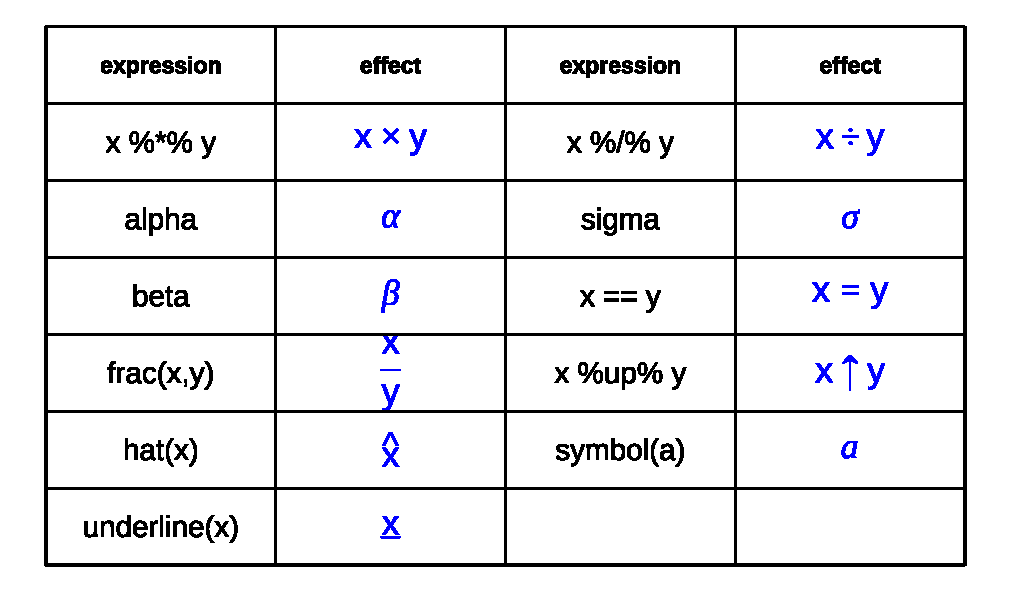
\includegraphics[width = 1\linewidth]{01.pdf}
      \end{figure}
        
        \begin{R}
a2 <- c('x + y','x - y','x %/% y','x/y','x%+-%y','x%.%y',
         'x %*% y','x %~%y','x*y','x~y',
        'x == y','x != y','x %==% y','x %prop% y',
        'x >= y','x <= y',
        'x < y', 'x > y', 'x %=~% y','x %~~% y'
        )
plot_table(a2,2)
ggsave('02.pdf')
       \end{R}
          \begin{figure}[H]
      \centering
        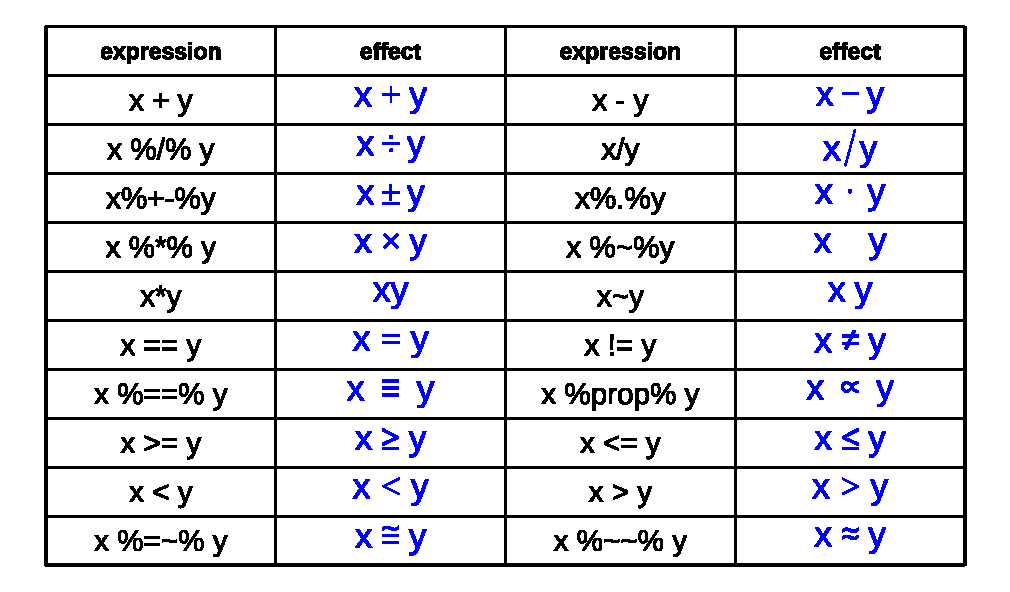
\includegraphics[width = 1\linewidth]{02.pdf}
      \end{figure}
     
     \begin{R}
a3 <- c('x[1]','x^2', 'sqrt(x)','sqrt(x,y)',
        'frac(x,y)', 'over(x,y)',
        'list(x,y,m,n)','!x',
        '...', '',
        'cdots','ldots', "paste(x,y)",'atop(x,y)'
        )
plot_table(a3,2)
ggsave('03.pdf')
     \end{R}
     \begin{figure}[H]
      \centering
        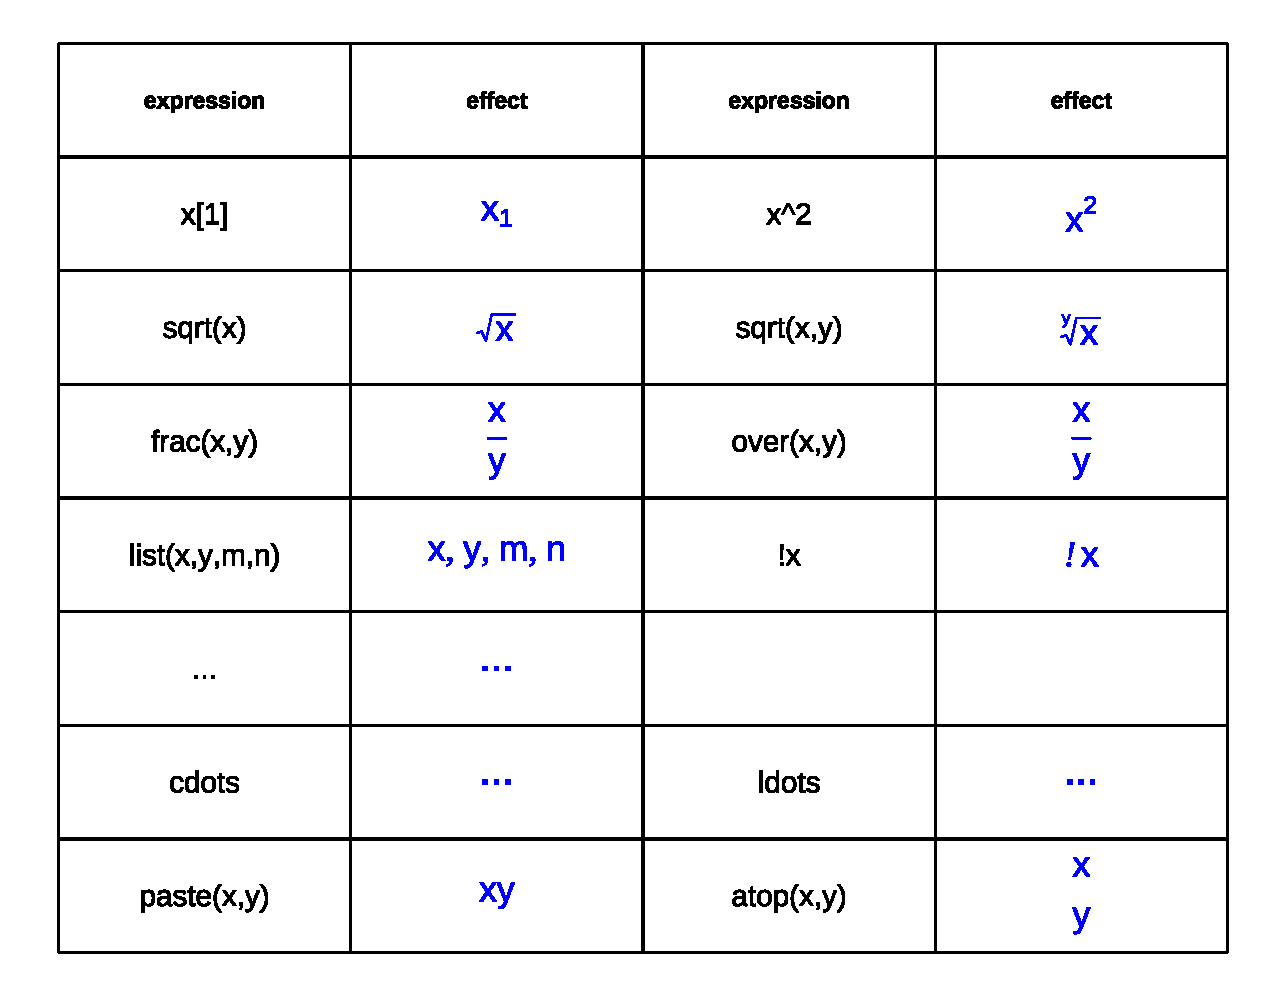
\includegraphics[width = 1\linewidth]{03.pdf}
      \end{figure}
     
     \begin{R}
a4 <- c('x %->% y','x %<-% y', 'x %<->% y', 'x %<=>% y',
        'x %=>% x', 'x %<=% y', 'x %up% y', 'x %down% y',
        'x %dblup% y','x %dbldown% y'
)
plot_table(a4,2)
ggsave('04.pdf')
     \end{R}
     
     \begin{figure}[H]
      \centering
        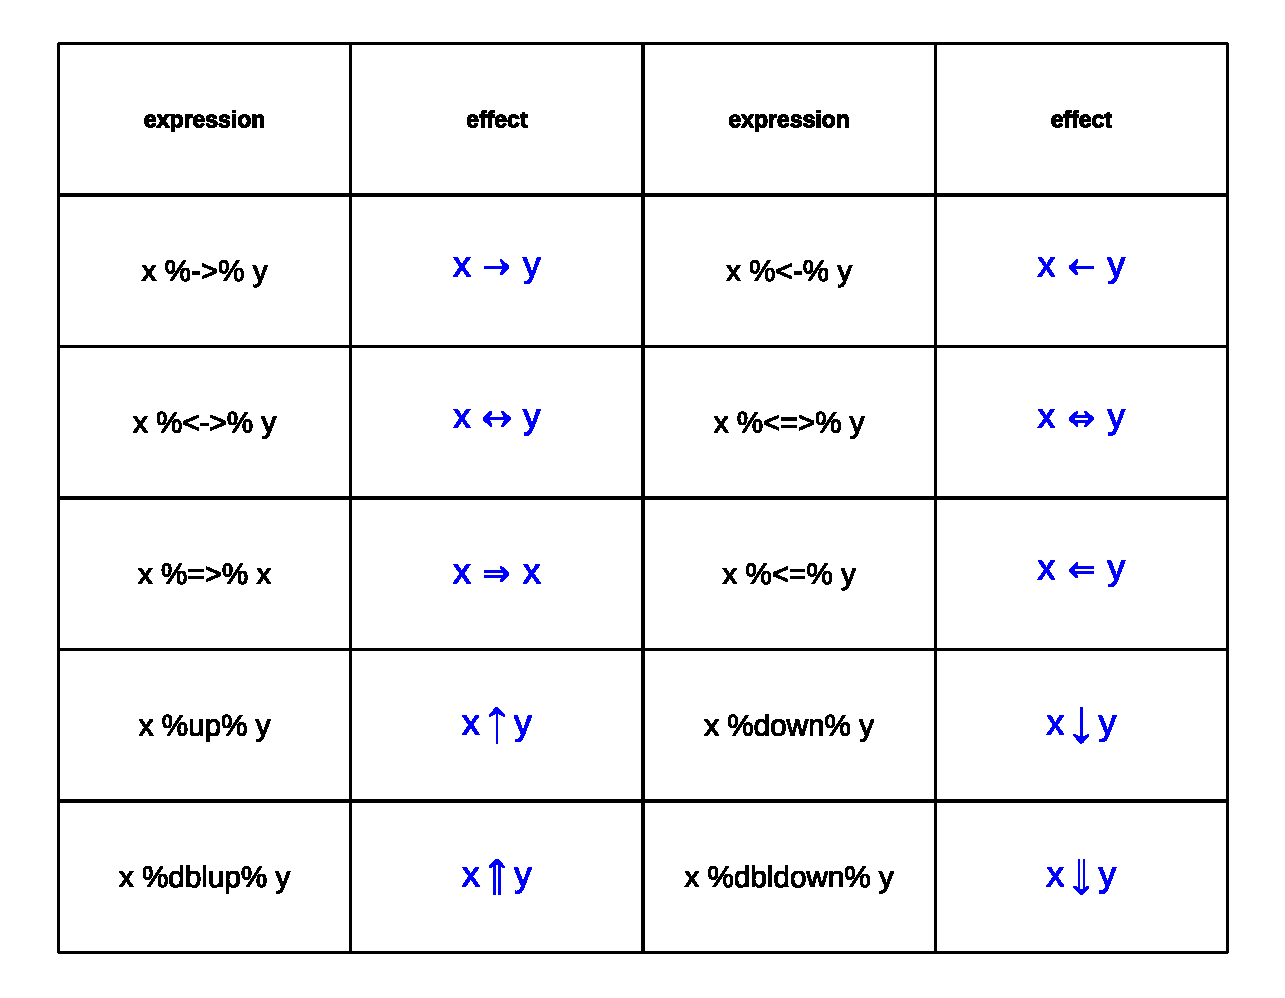
\includegraphics[width = 1\linewidth]{04.pdf}
      \end{figure}
      
      \begin{R}
a5 <- c('plain(x)','italic(x)','bold(x)','bolditalic(x)',
        'textstyle(x)','displaystyle(x)',
        'scriptstyle(x)', 'scriptscriptstyle(x)'
)
plot_table(a5,2)
ggsave('05.pdf')
      \end{R}
      \begin{figure}[H]
      \centering
        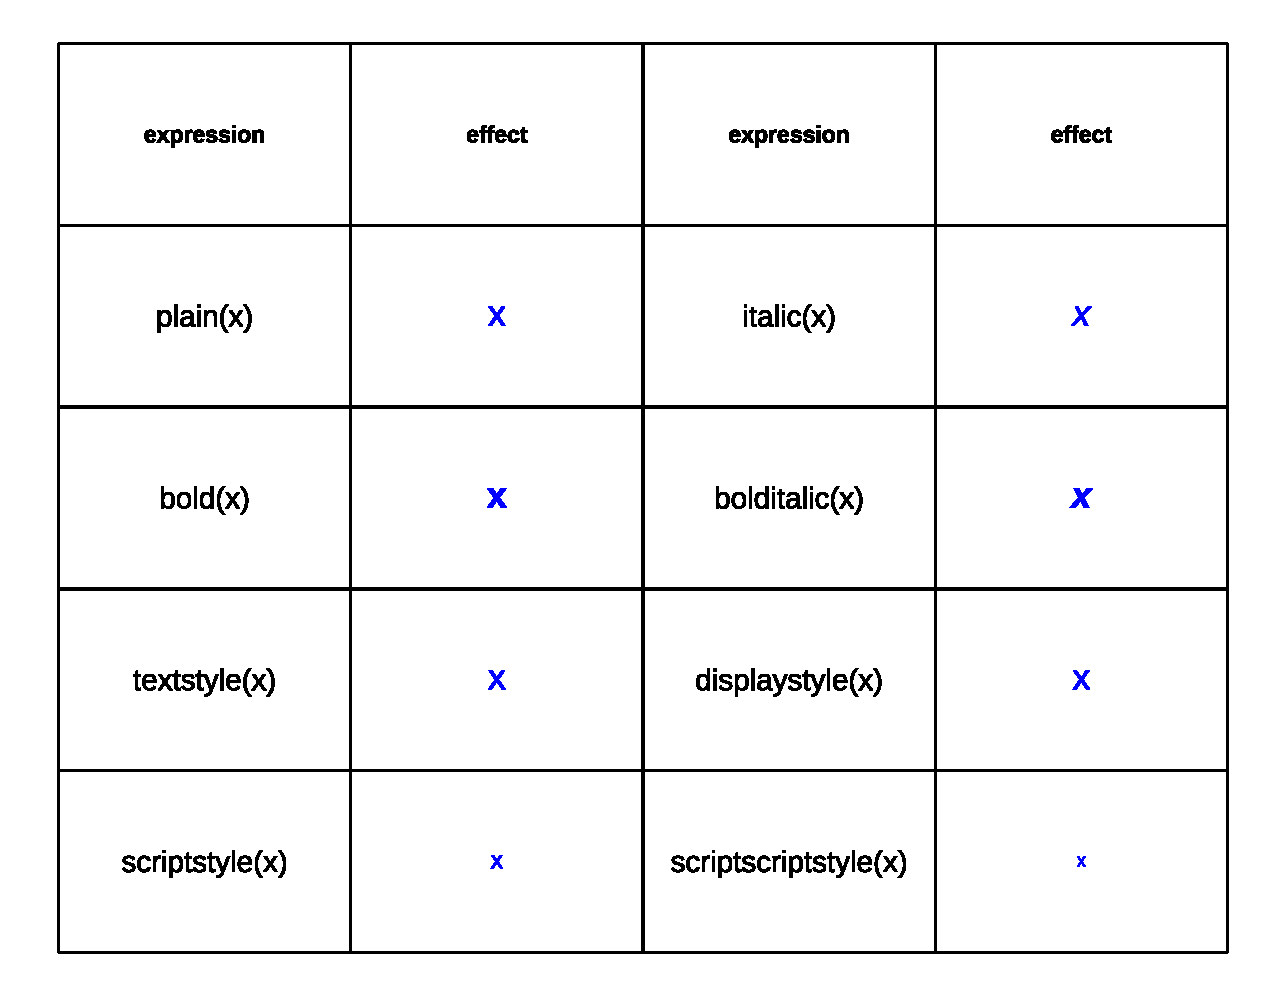
\includegraphics[width = 1\linewidth]{05.pdf}
      \end{figure}
     
     \begin{R}
a6 <- c('bar(x)', 'underline(x)','hat(x)','tilde(x)',
        'dot(x)','ring(x)',
        'widehat(xyz)','widetilde(xy)')
plot_table(a6,2)
ggsave('06.pdf')    
     \end{R} 
     \begin{figure}[H]
      \centering
        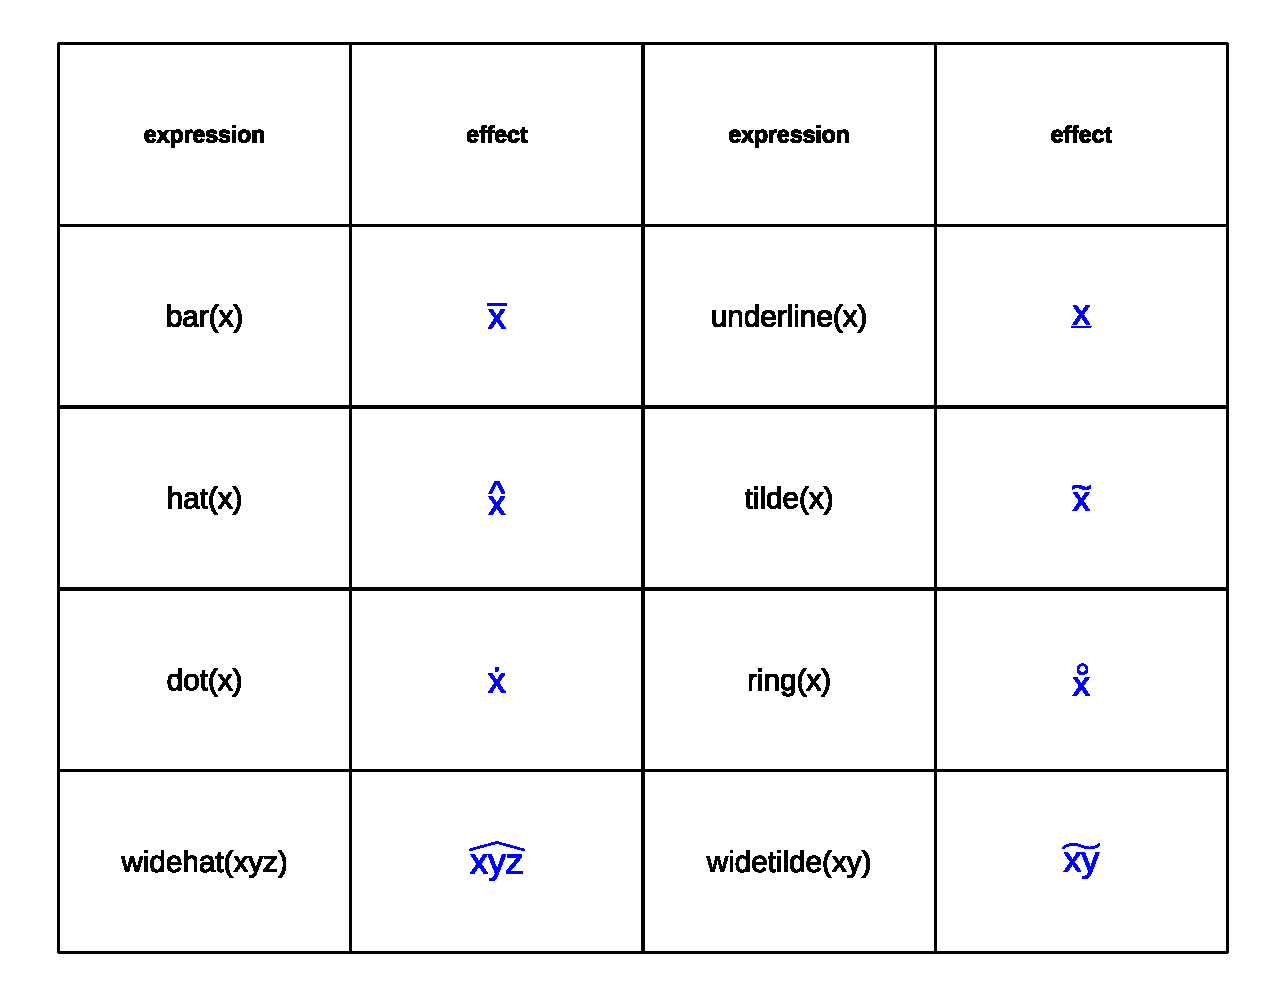
\includegraphics[width = 1\linewidth]{06.pdf}
      \end{figure}
      
      \begin{R}
a7 <- c('x %subset% y', 'x %subseteq% y', 'x %supset% y','x %supseteq% y',
        'x %notsubset% y', 'infinity', 'x %in% y',
        'x %notin% y')
plot_table(a7,2)
ggsave('07.pdf')
      \end{R}
      
      \begin{figure}[H]
      \centering
        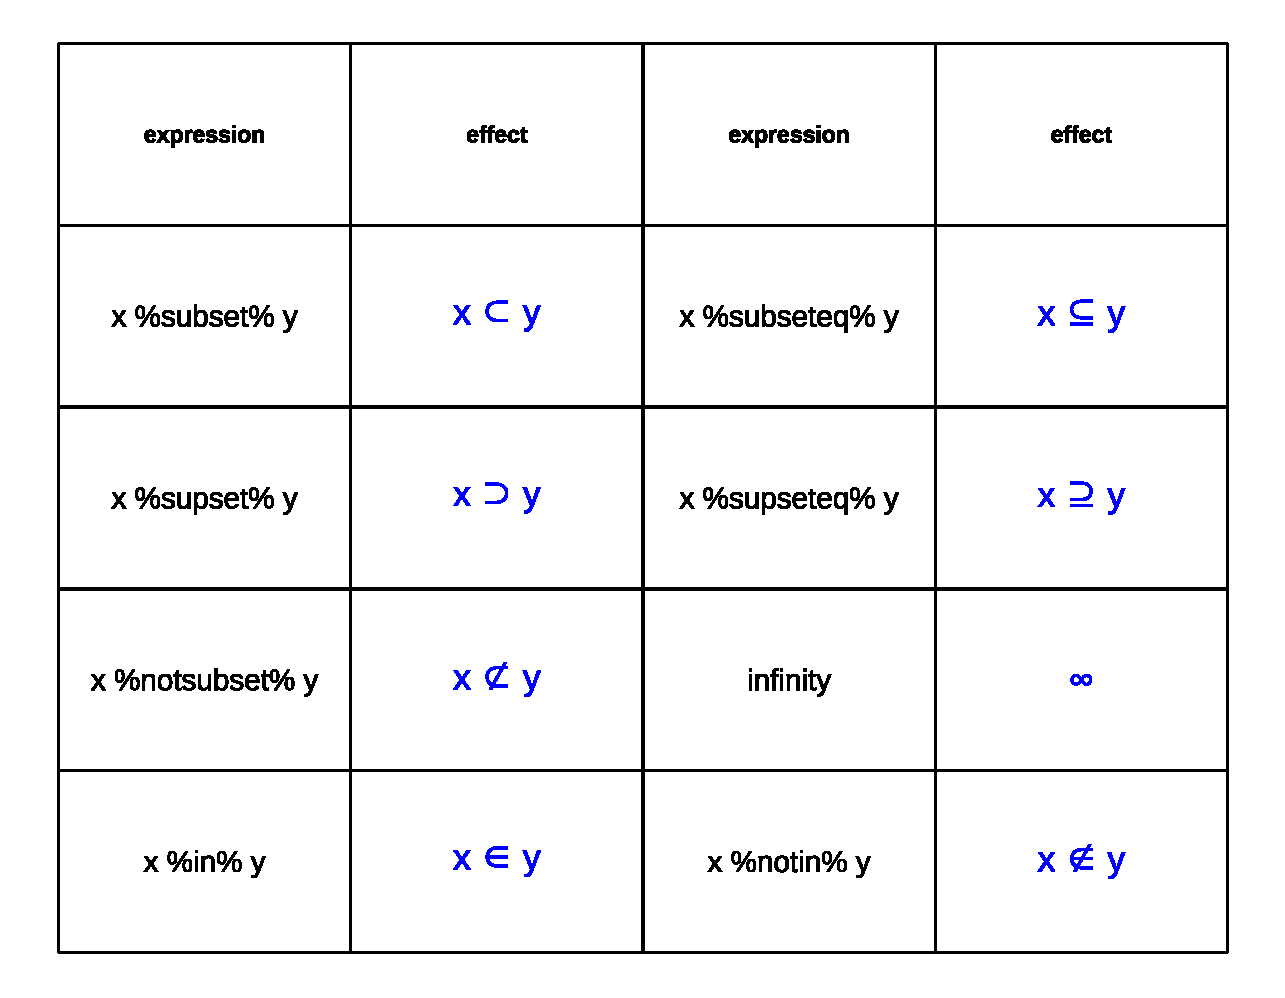
\includegraphics[width = 1\linewidth]{07.pdf}
      \end{figure}
      
      \begin{R}
a8 <- c('sum(f(x),a,b)','integral(f(x)*d(x),a,b)',
        'lim(f(x),x%->%5)','min(f(x),x >= 6)',
        'prod(f(x),a,b)',"bgroup('(',atop(x,y),')')"
)
plot_table(a8,1)
ggsave('08.pdf')
      \end{R}
      
      \begin{figure}[H]
      \centering
        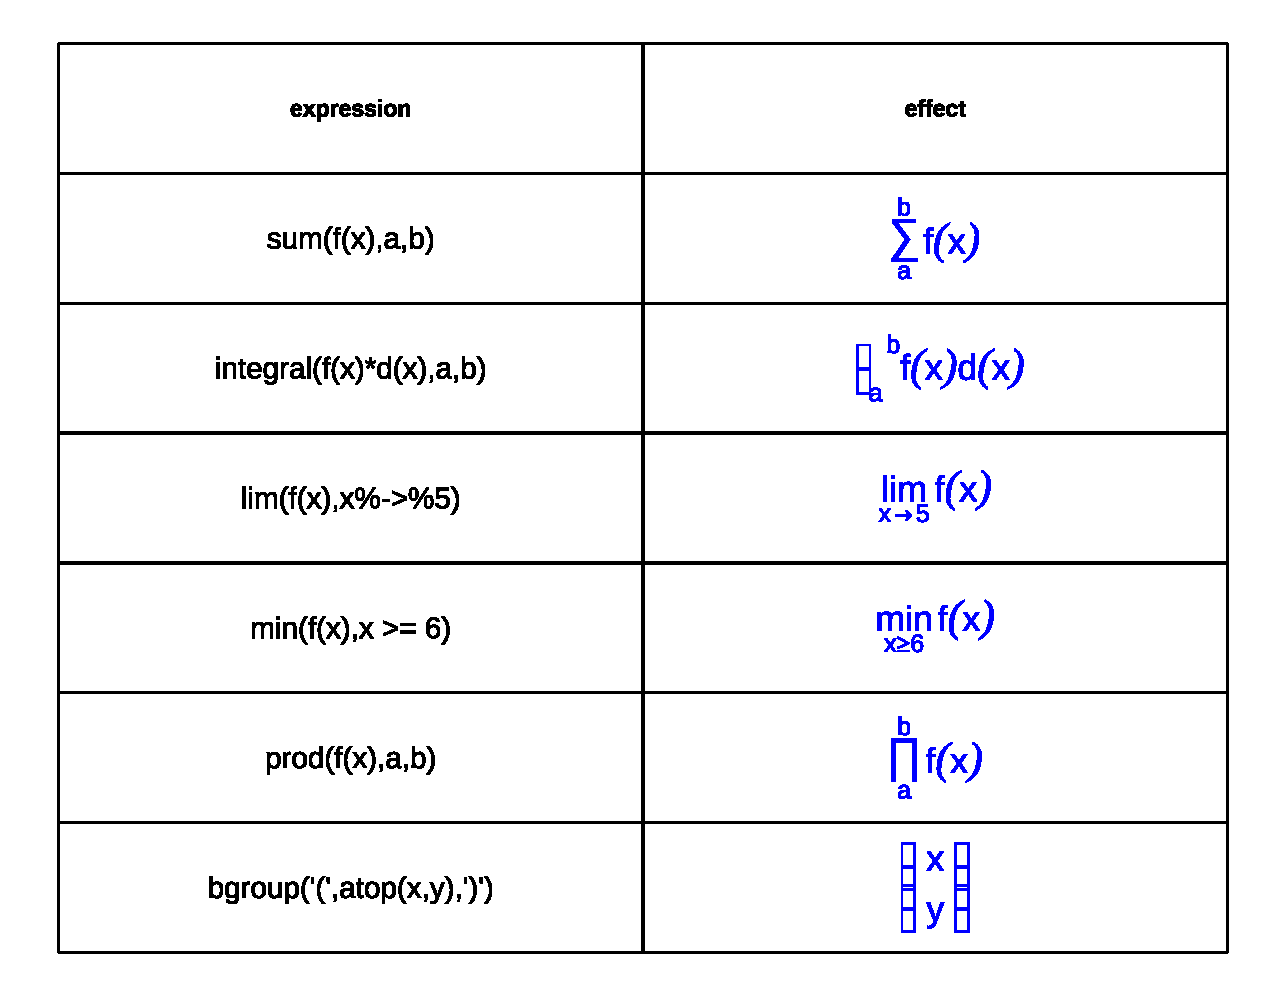
\includegraphics[width = 1\linewidth]{08.pdf}
      \end{figure}
      
      \begin{R}
a9 <- c('infinity',' partialdiff',
        'nabla', '9 * degree',
        '25 * minute', '60 * second')
plot_table(a9,2)
ggsave('09.pdf')
     \end{R}
     
     \begin{figure}[H]
      \centering
        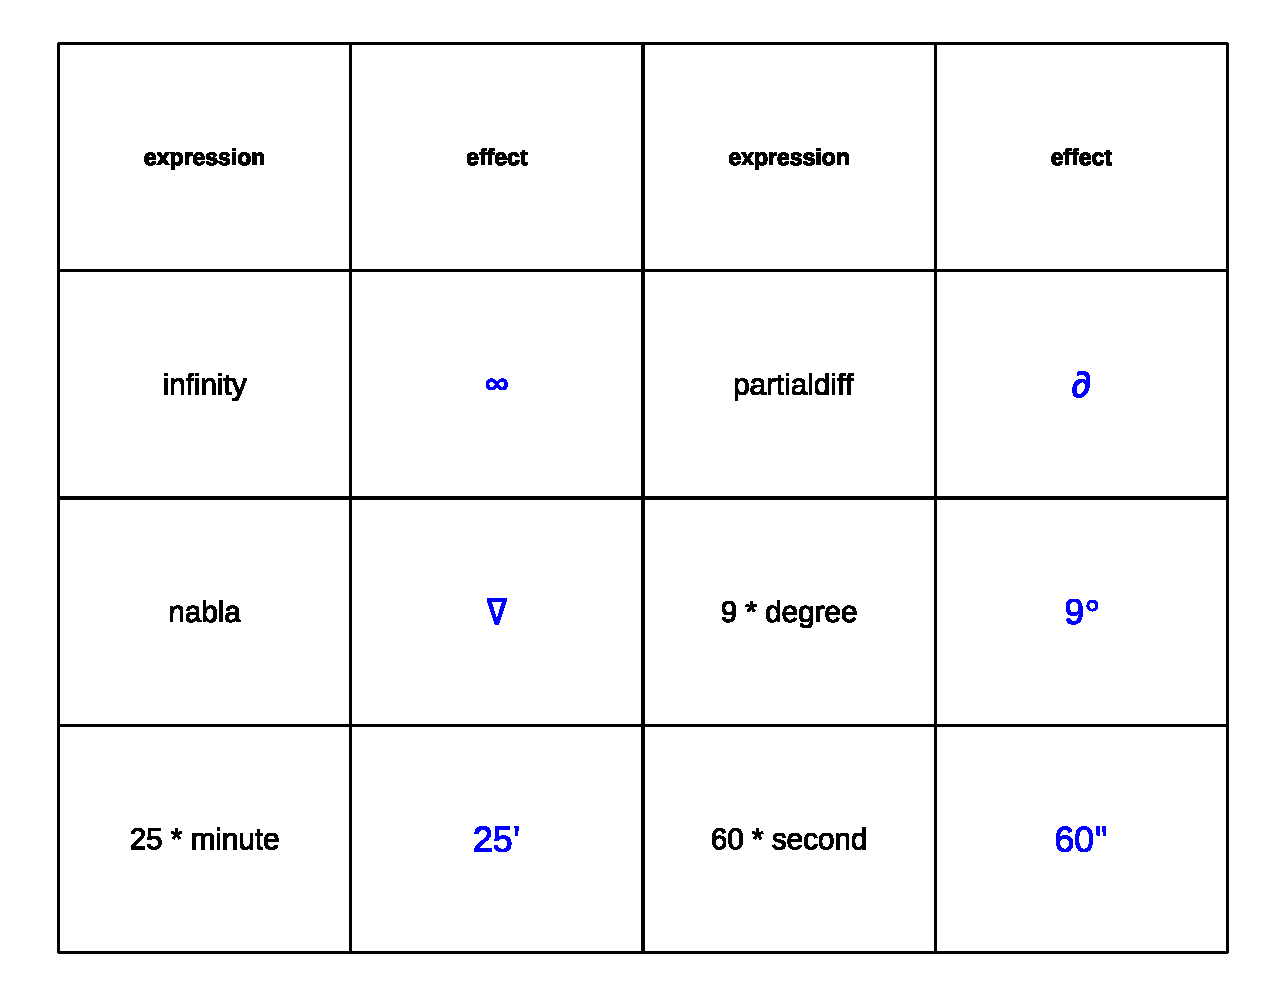
\includegraphics[width = 1\linewidth]{09.pdf}
      \end{figure}  
      
      \begin{R}
a10 <- c(paste0('symbol(',letters[1:26],')'),
         paste0('symbol(',LETTERS[1:26],')')
         )
plot_table(a10,2,F)
ggsave('10.pdf')
     \end{R}

   \begin{figure}[H]
      \centering
        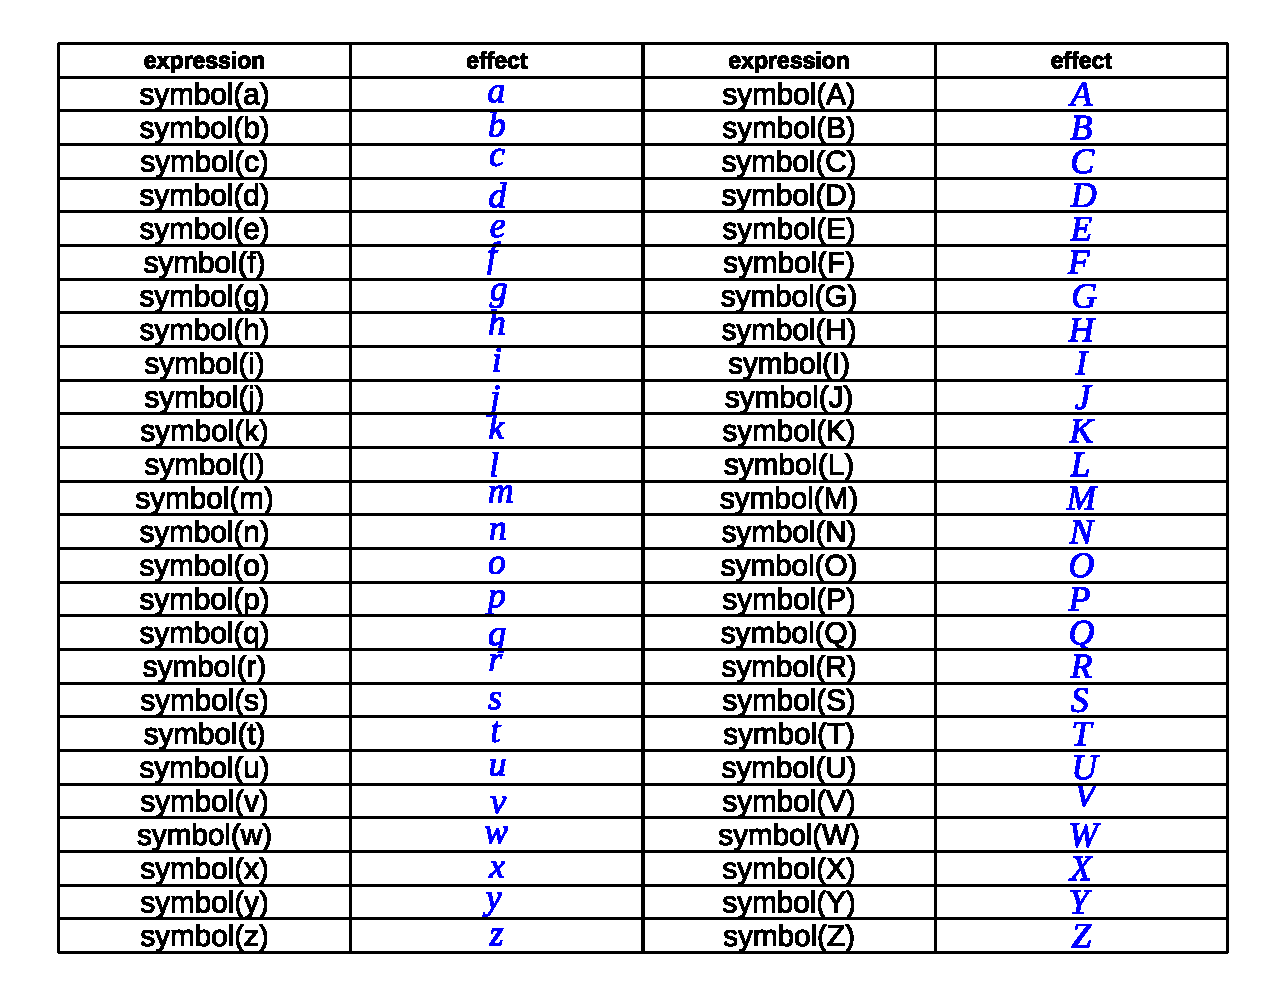
\includegraphics[width = 1\linewidth]{10.pdf}
      \end{figure}
      
      \begin{R}
a11 <- c('alpha','beta','chi','delta','epsilon',
         'eta','gamma','kappa','lambda','mu','nu',
          'omega',
          'phi', 'pi','psi','sigma','tau','upsilon',
         'varphi','xi','zeta')
library(Hmisc)
capitalize(a11) -> a12
plot_table(c(a11,a12),2,F)
ggsave('11.pdf')
          \end{R}
          
          \begin{figure}[H]
      \centering
        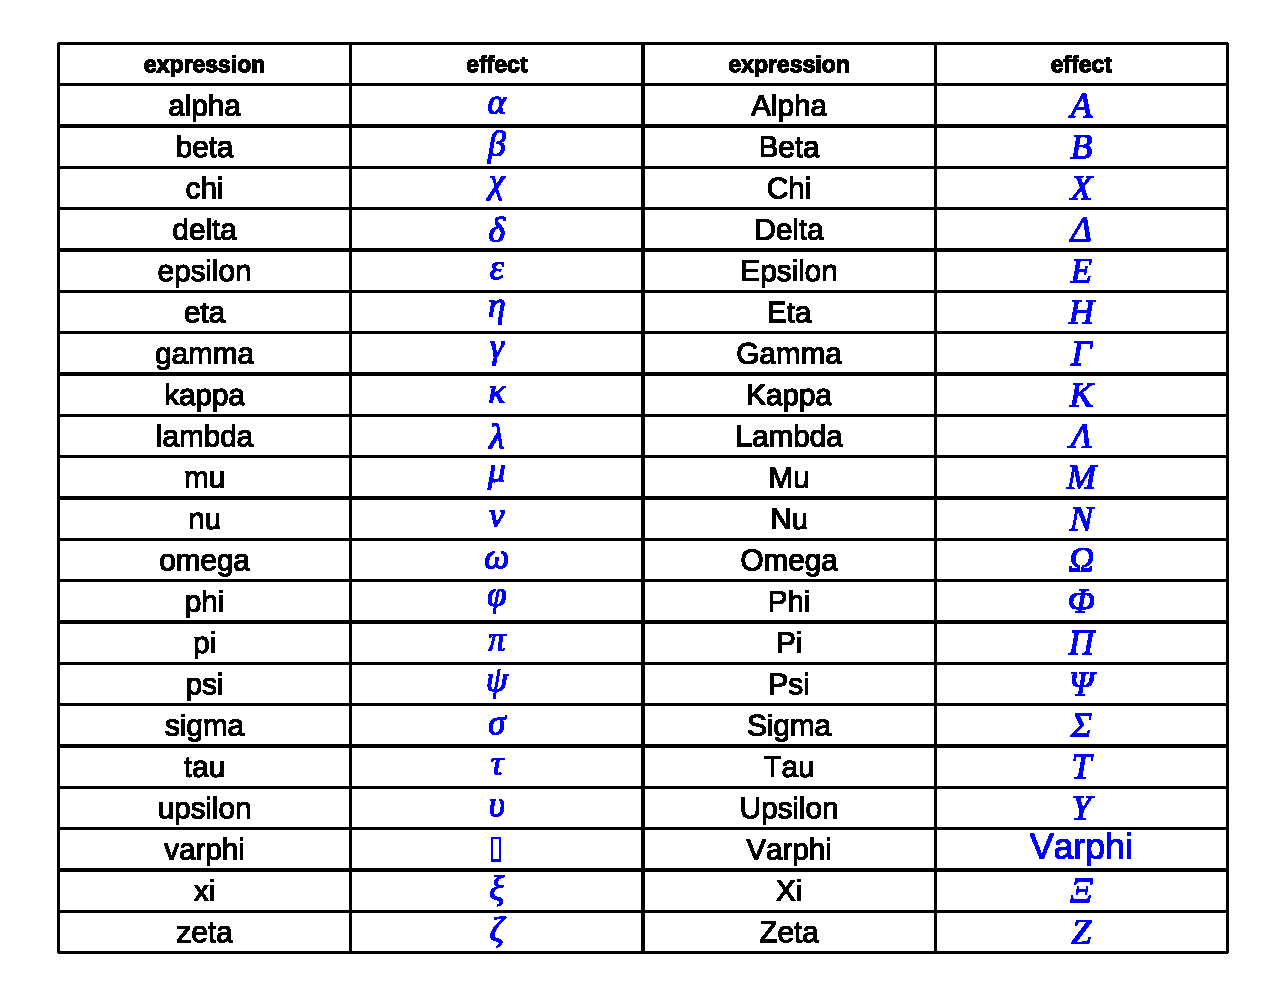
\includegraphics[width = 1\linewidth]{11.pdf}
      \end{figure}
      
      
\end{multicols*}

\end{document}